\documentclass[sigplan,10pt,review,anonymous]{acmart}
\settopmatter{printfolios=true,printccs=false,printacmref=false}

%% Some recommended packages.
\usepackage{booktabs}   %% For formal tables:
                        %% http://ctan.org/pkg/booktabs
\usepackage{subcaption} %% For complex figures with subfigures/subcaptions
                        %% http://ctan.org/pkg/subcaption

\usepackage[english]{babel}
\usepackage{bookmark}
\usepackage[utf8]{inputenc}
\usepackage[T1]{fontenc}
% \usepackage{lmodern}
\usepackage{xspace}
\usepackage{fancyhdr}
\usepackage{tcolorbox}

% Haskell code snippets and useful shortcuts
\usepackage{minted}
\setminted[haskell]{escapeinside=@@}
\newcommand{\hs}{\mintinline{haskell}}
\newcommand{\subhs}{\mintinline[fontsize=\small]{haskell}}
\newcommand{\cmd}[1]{\textsf{\color[rgb]{0,0,0.5} #1}}
\newcommand{\teq}{\smaller $\sim$}
\newcommand{\ghci}{$\lambda$>}
\newcommand{\defeq}{\stackrel{\text{def}}{=}}
\newcommand{\dollar}{{\color[rgb]{0.40,0.40,0.40} \$}}
\newcommand{\std}[1]{{\color[rgb]{0,0.3,0} #1}}
\newcommand{\blk}[1]{{\color[rgb]{0,0,0} #1}}
\newcommand{\blu}[1]{{\color[rgb]{0,0,1.0} #1}}

% Questions and tasks
\newcommand{\q}[2]{\textbf{\color{blue} Question #1:} #2}
\newcommand{\todo}[2]{[\textbf{\color{red} #1:} #2]}

%%
%% \BibTeX command to typeset BibTeX logo in the docs
\AtBeginDocument{%
  \providecommand\BibTeX{{%
    \normalfont B\kern-0.5em{\scshape i\kern-0.25em b}\kern-0.8em\TeX}}}

\setcopyright{none}
\bibliographystyle{ACM-Reference-Format}
\citestyle{acmauthoryear}

\makeatletter
  \defineshorthand[english]{"/}{\babelhyphen{nobreak}}
  \addto\extrasenglish{
    \languageshorthands{english}
    \useshorthands{"}
  }
\makeatother

\begin{document}

\title[Formal Verification of Spacecraft Control Programs]{Formal Verification
of Spacecraft Control Programs: An Experience Report}

\author{Andrey Mokhov}
\affiliation{
%   \department{School of Engineering}
  \institution{Newcastle University}
%   \city{Newcastle upon Tyne}
  \country{United Kingdom}
}
\email{andrey.mokhov@ncl.ac.uk}
\author{Georgy Lukyanov}
\affiliation{
%   \department{School of Engineering}
  \institution{Newcastle University}
%   \city{Newcastle upon Tyne}
  \country{United Kingdom}
}
\email{g.lukyanov2@ncl.ac.uk}
\author{Jakob Lechner}
\affiliation{
%   \department{School of Engineering}
  \institution{RUAG Space GmbH}
%   \city{Newcastle upon Tyne}
  \country{Austria}
}
\email{jakob.lechner@gmx.net}

% \fancypagestyle{firstpagestyle}
% {
%    \fancyhf{}
%    \renewcommand{\headrulewidth}{0.2pt}
%    \fancyhead[C]{Under review, feedback is sought}
% }

\begin{abstract}
Verification of correctness of control programs is an essential task
in the development of space electronics; it is difficult and typically
outweighs design and programming tasks in terms of development hours.
This experience report presents a verification approach designed to help
spacecraft engineers reduce the effort required for formal verification of
low-level control programs executed on custom hardware.

% The approach uses a
% metalanguage to describe the semantics of a program as a state transformer,
% which can be compiled to multiple targets for testing, formal verification, and
% code generation. The metalanguage is embedded in Haskell, providing a way to
% prove some properties at the type level, which can shorten the feedback loop
% and further increase the productivity of engineers.

The verification approach is demonstrated on an industrial case study.
We present REDFIN, a processing core used in space missions, and its formal
semantics expressed using the proposed metalanguage for state transformers,
followed by examples of verification of simple control programs.

\keywords{formal verification, instruction set architecture, functional
programming, domain-specific languages.}
\end{abstract}

\maketitle

\section{Introduction}

Software bugs play a major role in the history of spacecraft
accidents~\cite{Leveson2004}. There are recorded cases of mission-ending bugs
that would have been difficult to prevent (e.g. caused by concurrency
or updates) but also plain integer overflows~\cite{bug-rocket} and incorrect unit
conversion~\cite{NASA:1999:Mars}, which should have been eradicated long ago.

Alas, there is no silver bullet. Testing is supported by mature methodologies
and frameworks, but does not provide the full correctness guarantee. General-purpose
strongly-typed languages can be used to eliminate important classes of bugs, but
are less familiar to software engineers and are often not suitable for highly
resource-constrained microarchitectures used in space electronics. Formal modelling
methods provide a systematic approach for developing complex systems in a
correct-by-construction manner, but they are still at the bleeding-edge of
computing science and can be difficult to apply to real-life systems. This paper
combines known formal verification and programming languages techniques and presents
a formal verification approach for simple control tasks, such as satellite power
management, which are executed on a real processing core used in space missions.
We believe the presented ideas are transferable to other domains with similar
safety and resource requirements, e.g. biomedical applications.
\begin{figure}
\centerline{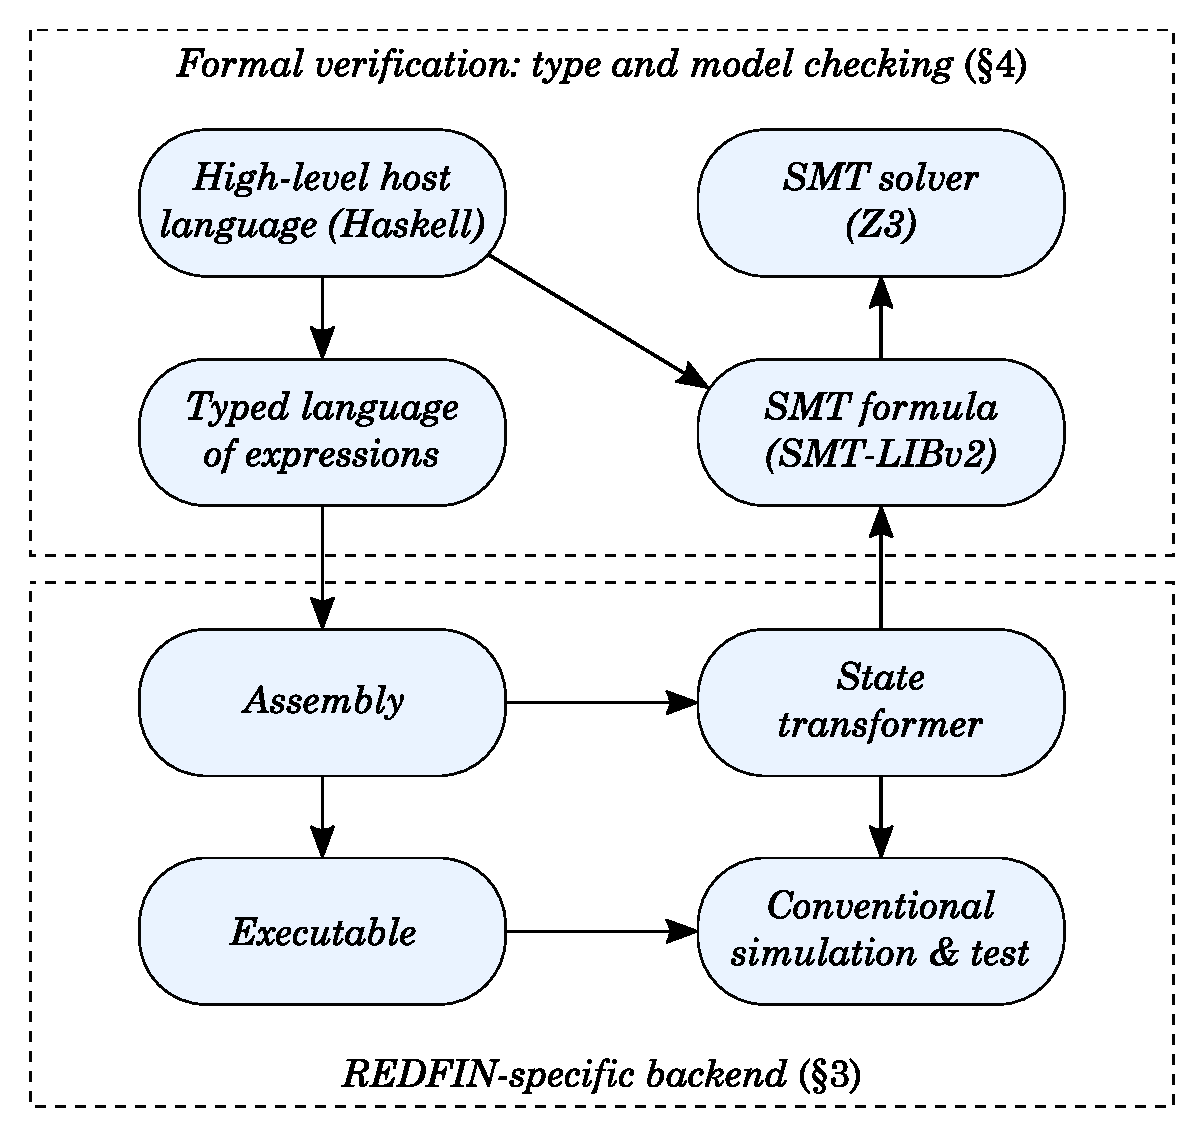
\includegraphics[scale=0.45]{fig/overview.pdf}}

\caption{Overview of the presented formal verification approach.\label{fig-overview}}

\end{figure}

Fig.~\ref{fig-overview} shows an overview of the presented approach. The bottom
part corresponds to conventional code generation and simulation, where
REDFIN\footnote{REDFIN stands for `REDuced instruction set for Fixed-point \&
INteger arithmetic'. This instruction set and the corresponding processing core
were developed by RUAG Space Austria GmbH for space missions.
See~\S\ref{sec-redfin} for more details.} assembly language is executed by
simulating the effect of each instruction on the state of the processor and memory.
The corresponding \emph{state transformer} is typically implicit and intertwined
with the rest of the simulation infrastructure. The main idea of our approach is
to represent the state transformer explicitly so that it can be symbolically
manipulated and used not only for simulation but also for formal verification by
compiling it into an SMT formula. We can then~use~an~SMT solver, e.g.
Z3~\cite{de2008z3}, to verify that the state transformer of a given program
satisfies certain properties, for example, that integer overflow cannot occur
regardless of input parameters and that the program always terminates within
given time.

By embedding the state transformer metalanguage in Haskell we can readily
implement compilers from higher-level \emph{typed} languages to untyped assembly,
eradicating incorrect number and unit conversion bugs. As shown at the top of
Fig.~\ref{fig-overview}, engineers can write high-level control
programs for the REDFIN architecture directly in a small subset of Haskell. These
high-level programs can be used for type-safe code generation and as executable
specifications of intended functionality for the purposes of program synthesis and
equivalence checking. % (\S\ref{sec-verification}).

We first introduce the REDFIN processing core (\S\ref{sec-redfin}), and then
describe and discuss the presented approach
(\S\ref{sec-transformer}-\S\ref{sec-discussion}). Related work is reviewed
in~\S\ref{sec-related}.

\clearpage

\vspace{-1mm}
\section{The REDFIN architecture overview\label{sec-redfin}}
\vspace{-0.5mm}
% For many spacecraft subsystems integrated circuits are required to perform control
% tasks or simple data processing. Typically, these integrated circuits are realised
% with FPGAs (Field Programmable Gate Arrays) due to their flexibility and lower
% costs compared to ASIC (Application-Specific Integrated Circuit) development \&
% fabrication. Since FPGAs can be used to implement arbitrary circuit functions
% including processor cores, it is possible to perform tasks both in hardware and
% in software. However, modern space-qualified FPGAs, which can withstand radiation
% in Earth orbit or deep space, have a limited amount of programmable resources.
% Therefore, it is often not feasible to implement a fully-fledged processor system
% in such an FPGA next to the mission-specific circuitry.

Many spacecraft subsystems rely on integrated circuits to perform control tasks
or simple data processing. Typically, these integrated circuits are realised
with Field Programmable Gate Arrays (FPGAs) benefiting from their flexibility
and low cost. Modern space-qualified FPGAs that can withstand radiation in Earth
orbit or deep space have a limited amount of programmable resources, and it is
often not feasible to implement a fully-fledged processor system in such an FPGA
next to the mission-specific circuitry.
The REDFIN instruction set was developed to address this issue and meet the
following goals: (i)~simple instruction set with a small hardware footprint,
(ii)~reduced complexity to support formal verification of programs, and
(iii)~deterministic real-time behaviour.

\subsection{REDFIN instruction set and microarchitecture}
\vspace{-0.5mm}

REDFIN instructions have a fixed width of 16 bits.
The instruction set is based on a register-memory architecture, i.e.
instructions can fetch their operands from registers as well as directly from the
memory. This architecture favours a small register set, which minimises the hardware
footprint of the processing core. Furthermore, the number of instructions in a
program is typically smaller in comparison to traditional load/store architectures
where all operands have to be transferred to registers before any operations can
be performed. There are 47 instructions of the following types:

\vspace{-0.5mm}
\begin{itemize}
\item{Load/store instructions for moving data between registers and memory, and
loading of immediate values.}
\item{Integer and fixed-point arithmetic operations.}
% In the latter
% case the number of fractional bits can be adjusted by a processor register.
\item{Bitwise logical and shift operations.}
\item{Control flow instructions and comparison operations.}
\item{Bus access instructions for read \& write operations on an AMBA AHB bus
(not covered in this paper).}
\end{itemize}
\vspace{-0.5mm}

The REDFIN processing core fetches instruction and data words from a small and fast
on-chip SRAM. This only allows for execution of simple programs, however, it also
eliminates the need to implement caches and thus removes a source of non-determinism of
conventional processors. High performance is not one of the main goals, hence the
core is not pipelined and does not need to resolve data/control hazards or
perform any form of speculative execution. These properties greatly simplify
worst case execution time analysis.

\vspace{-1.2mm}
\subsection{Requirements for formal verification}
\vspace{-0.5mm}

Verification of \emph{functional correctness} of REDFIN programs, as defined by a
requirement specification, clearly is an essential task for the development of space
electronics. There are also important \emph{non-functional requirements}, such as
worst case execution time and energy consumption, which rely on the implementation
guarantees provided by the processing core. To reduce verification complexity,
the REDFIN core only allows to execute a single subroutine whose execution is triggered
by a higher-level controller in the system. The implementation guarantees that
concurrent bus accesses to the processor registers or memory do not affect
the subroutine execution time. Furthermore, the processor does not implement
interrupt handling. All these measures are taken to provide real-time
subroutine execution guarantees and make the verification of non-functional
properties feasible. % within the presented verification framework.

Despite these restrictions the REDFIN core has already proven its effectiveness for
simple control tasks and arithmetic computations as part of an antenna pointing unit
for satellites. Nevertheless, verification can be difficult and time-consuming,
even for small and simple programs. Verification activities, following engineering
standards for space electronics, typically outweigh programming and design tasks by a
factor of two in terms of development hours. Usually verification is performed via
program execution on an instruction set simulator or a hardware model of the processor.
Manually deriving test cases from the specification is cumbersome and error-prone
and simulation times can become prohibitively long with a large number of tests that
are often needed to reach the desired functional and code coverage. Formal verification
methods can prove that a program satisfies certain properties for all possible
test cases and are therefore immensely valuable for completing the verification
with superior efficiency and quality.


\vspace{-1.5mm}
\section{Modelling REDFIN in Haskell\label{sec-transformer}}
\vspace{-1mm}

In this section we formally define the REDFIN microarchitecture and express the
semantics of the instruction set as an explicit and symbolic state transformer.


\subsection{The REDFIN microarchitecture state}


The main idea of the presented approach is to use an explicit state"/transformer
semantics of the REDFIN microarchitecture. The state space of the entire
processing core is a Cartesian product of state spaces of every component:

\begin{equation}
\begin{split}
S=\{(r, m, ic, ir, p, f, c) : r \in R, m \in M, ic \in A, ir \in I,\\
p \in P, f \in F, c \in C\},
\end{split}
\end{equation}

\noindent
where $R$ is the set of register bank configurations;
$M$ is the memory state space;
$A$~is the set of instruction addresses (the instruction counter $ic$ stores the
address of the current instruction);
$I$ is the set of instruction codes (the instruction register $ir$ stores the
code of the current instruction);
$P$ is the set of programs;
$F$ is the set of the flag register configurations; and
$C$ is the set of clock values.

Fig.~\ref{fig-types} shows the translation of the above into Haskell types. Note
that the types are not parameterised: recall that REDFIN is parameterised, e.g.
the data width can be chosen depending on mission requirements, whereas we use fixed
64-bit data path for the sake of simplicity. The chosen names are self-explanatory,
for example, the data type \hs{State} directly corresponds to the set of states~$S$.
We defined \hs{SymbolicValue} and \hs{SymbolicArray} type constructors on top of
Levent Erkok's symbolic verification library SBV~\cite{SBV}, which we use as the
SMT translation and verification frontend. In principle, any other SMT frontend
can be used, but to the best of our knowledge, SBV is the most mature SMT library
available for Haskell. We briefly overview all \hs{State} components below.

\begin{figure}[t]

\begin{minted}{haskell}
data State = State
  { registers           :: RegisterBank
  , memory              :: Memory
  , instructionCounter  :: InstructionAddress
  , instructionRegister :: InstructionCode
  , program             :: Program
  , flags               :: Flags
  , clock               :: Clock }
\end{minted}

\begin{minted}{haskell}
type Register           = SymbolicValue Word2
type Value              = SymbolicValue Int64
type RegisterBank       = SymbolicArray Word2 Int64
\end{minted}

\begin{minted}{haskell}
type MemoryAddress      = SymbolicValue Word8
type Memory             = SymbolicArray Word8 Int64
\end{minted}

\begin{minted}{haskell}
type InstructionAddress = SymbolicValue Word8
type InstructionCode    = SymbolicValue Word16
type Program            = SymbolicArray Word8 Word16
\end{minted}

\begin{minted}{haskell}
data Flag               = Condition | Overflow | ...
type Flags              = SymbolicArray Flag Bool
\end{minted}

\begin{minted}{haskell}
type Clock              = SymbolicValue Word64
\end{minted}

\caption{Basic types for encoding REDFIN microarchitecture in Haskell.\label{fig-types}}

\end{figure}


\subsubsection{Data values, registers and memory}
64-bit data values (\hs{Int64}) are stored in registers and memory. There are~4
registers (addressed by \hs{Word2}) and 256 memory locations (addressed by
\hs{Word8}). Their content is represented by symbolic arrays that can be
accessed via SBV's functions \hs{readArray} and \hs{writeArray}.


\subsubsection{Instructions and programs}
REDFIN instructions are represented by 16-bit \hs{InstructionCode}, whose 6
leading bits contain the instruction opcode, and the remaining 10 bits are
allocated for various instruction arguments. The \hs{Program} is a symbolic
array mapping 8-bit instruction addresses to instruction codes.


\subsubsection{Status flags and clock}
The microarchitecture stores execution status flags to support conditional
branching, track integer overflow, and terminate the program, as captured by the
data type \hs{Flag} (we omit a few other flags for brevity). The flag register is a
symbolic map from flags to Boolean values. The \hs{Clock} is a 64-bit counter
incremented on each clock cycle. Status flags and the clock are used for
diagnostic, formal verification and worst-case execution time analysis.


\subsection{Instruction and program semantics}

We can now define the formal semantics of REDFIN instructions and programs in terms
of a \emph{state transformer} $T : S \rightarrow S$, i.e. a function that maps
states to states. We distinguish between instructions and programs by using
Haskell's list notation, for example, $T_{\subhs{nop}}$ is the semantics of the
instruction $\hs{nop} \in I$, whereas $T_{\subhs{[}\subhs{nop}\subhs{]}}$ is the
semantics of the single-instruction program $\hs{[}\hs{nop}\hs{]} \in P$.

% \footnote{REDFIN does not have a dedicated \hs{nop}
% instruction, but one can use the semantically equivalent instruction \hs{jmpi 0}
% instead (i.e. jump to the next instruction).}

\textbf{Definition (program semantics):} The semantics of a program $p \in P$
is inductively defined as follows:


\begin{itemize}
    \item The semantics of the \emph{empty program} $\hs{[}\hs{]} \in P$ coincides with
    the semantics of the instruction \hs{nop} and is the identity state transformer:
    $T_{\subhs{[}\subhs{]}} = T_{\subhs{nop}} = \hs{id}$.
    
    \item The semantics of the \emph{single-instruction program} $\hs{[}\hs{i}\hs{]} \in P$
    is a composition of three state transformers: (i) fetching the instruction from
    the program memory (denoted by $T_\textit{fetch}$), (ii) incrementing the
    instruction counter ($T_\textit{inc}$), and (iii) the state transformer
    of the instruction itself ($T_{\subhs{i}}$), that is:
    
    \[
    \begin{array}{lcl}
    T_\textit{fetch} & = & (r, m, ic, ir, p, f, c) \mapsto (r, m, ic, p[ic], p, f, c + 1)\\
    T_\textit{inc} & = & (r, m, ic, ir, p, f, c) \mapsto (r, m, ic + 1, ir, p, f, c)\\
    T_{\subhs{[}\subhs{i}\subhs{]}} & = & T_{\subhs{i}} \circ T_\textit{inc} \circ T_\textit{fetch}.\\
    \end{array}
    \]
    
    \item The semantics of the \emph{composite program} $\hs{i}\hs{:}\hs{p} \in P$,
    where the operator~\hs{:}~prepends an instruction $\hs{i} \in I$ to a program
    $\hs{p} \in P$, is defined as $T_{\subhs{i}\subhs{:}\subhs{p}} = T_{\hs{p}} \circ T_{\subhs{[}\subhs{i}\subhs{]}}$.
    
\end{itemize}

\noindent
We represent state transformers in Haskell using the \emph{state monad}, a
classic approach to emulating mutable state in a purely functional programming
language~\cite{wadler1990comprehending}. We call our state monad~\hs{Redfin} and
define it\footnote{\mbox{A generic version of this monad is available in standard module
\hs{Control.Monad.State}.}} as follows:


\begin{minted}{haskell}
data Redfin a = Redfin
  { transform :: State -> (a, State) }
\end{minted}


\noindent
Every computation with the return type~\hs{Redfin} \hs{a} yields a value of type~\hs{a}
and possibly alters the \hs{State} of the REDFIN microarchitecture. As an example,
below we express the state transformer $T_\textit{inc}$ using the \hs{Redfin} monad.


\begin{minted}{haskell}
incrementInstructionCounter :: Redfin ()
incrementInstructionCounter =
  Redfin $ \current -> ((), next)
  where
    next = current { instructionCounter =
      instructionCounter current + 1 }
\end{minted}


\noindent
In words, the state transformer looks up the value of the \hs{instructionCounter}
in the \hs{current} state and replaces it in the \hs{next} state with the
incremented~value. The type \hs{Redfin ()} indicates that the computation does not
produce any value as part of the state transformation. Such computations directly
correspond to REDFIN programs and can be composed using the operator \hs{>>}.
For example, \hs{fetchInstruction}\\\hs{>>}~\hs{incrementInstructionCounter} is
the state transformer $T_\textit{inc} \circ T_\textit{fetch}$ assuming that
\hs{fetchInstruction} corresponds to $T_\textit{fetch}$. We can also use
Haskell's powerful \hs{do}-notation to compose computations:


\begin{minted}{haskell}
readInstructionRegister :: Redfin InstructionCode
readInstructionRegister =
  Redfin $ \s -> (instructionRegister s, s)
\end{minted}

\begin{minted}{haskell}
executeInstruction :: Redfin ()
executeInstruction = do
  fetchInstruction
  incrementInstructionCounter
  instructionCode <- readInstructionRegister
  decodeAndExecute instructionCode
\end{minted}

\noindent
Here \hs{readInstructionRegister} extracts the instruction code from the current
state \emph{without modifying it}. This function is used in \hs{executeInstruction},
which defines the semantics of the REDFIN execution cycle. We omit the definition of
\hs{decodeAndExecute} for brevity: it is a case analysis of 47 opcodes that returns
the matching instruction. We introduce several interesting instructions below.


\subsubsection{Halting the processor}
If the~\hs{halt} instruction is encountered, the processor sets the flag~\hs{Halt},
thereby stopping the execution of the current subroutine until a new one is
started by a higher-level system controller that resets \hs{Halt}. The auxiliary
function \hs{writeFlag} is used to do the actual flag modification.


\begin{minted}{haskell}
halt :: Redfin ()
halt = writeFlag Halt true
\end{minted}

\begin{minted}{haskell}
writeFlag :: Flag -> SymbolicValue Bool -> Redfin ()
writeFlag flag value = Redfin $ \s -> ((), s')
  where s' = s { flags = writeArray (flags s)
                         (flagId flag) value }
\end{minted}



\subsubsection{Arithmetics}
As a more involved example, consider the semantics of the instruction \hs{abs}.
It reads a register and writes back the absolute value of its
contents\footnote{We use \hs{Prelude.abs} to distinguish between the instruction
and the function from the standard library \hs{Prelude}; \hs{fmap} applies
\hs{Prelude.abs} to the result of \hs{readRegister}.}.
The semantics accounts for the potential integer overflow that leads to the
\emph{negative resulting value} when the input is $-2^{63}$ (REDFIN
uses the two's complement signed number representation). The overflow is flagged
by setting~\hs{Overflow}.


\begin{minted}{haskell}
abs :: Register -> Redfin ()
abs rX = do
    state  <- readState
    result <- fmap Prelude.abs (readRegister rX)
    let (_, overflowState) =
      transform (writeFlag Overflow true) state
    writeState $ ite (result .< 0)
                     overflowState state
    writeRegister rX result
\end{minted}


\noindent
Here, SBV's symbolic \emph{if-then-else} operation~\hs{ite} is used to \emph{merge}
two possible next states, one of which has the \hs{Overflow} flag set. We use
auxiliary functions \hs{readRegister}, \hs{writeRegister}, \hs{readState} and
\hs{writeState} --- simple state transformers defined similarly to
\hs{readInstructionRegister} and \hs{writeFlag}.


\subsubsection{Conditional branching}
As an example of a control flow instruction, consider the conditional branching
instruction \hs{jmpi_ct}, which tests the~\hs{Condition} flag, and adds the
provided offset to the instruction counter if the flag is set.


\begin{minted}{haskell}
jmpi_ct :: SymbolicValue Int8 -> Redfin ()
jmpi_ct offset = do
  ic <- readInstructionCounter
  condition <- readFlag Condition
  let ic' = ite condition (ic + offset) ic
  writeInstructionCounter ic'
\end{minted}


\noindent
After working through the above examples, it is worth noting that we use our
Haskell encoding of the state transformer as a~\emph{metalanguage}. We are
operating the REDFIN core as a puppet master, using external
meta-notions of addition,
comparison and let"/binding. From the processor's
point of view, we have infinite memory and act instantly, which gives us unlimited
modelling power. For example, we can run a simulation of the processor environment
in an external tool and feed its result to \hs{writeRegister} as if it was
obtained in a single clock cycle.

\subsection{Symbolic simulation}

Having defined the semantics of REDFIN instructions and programs, we can
implement symbolic simulation of the processor:

\begin{minted}{haskell}
simulate :: Int -> State -> State
simulate steps s
    | steps <= 0 = s
    | otherwise  = ite halted
                       s (simulate (steps - 1) nextS)
  where
    halted = readArray (flags s) (flagId Halt)
    nextS  = snd $ transform executeInstruction s
\end{minted}

\noindent
The function takes a number of simulation steps $N$ and an initial symbolic
state of the processor as input, and executes $N$ instructions using the
previously defined \hs{executeInstruction} function. In each \hs{state} we need
to merge two possible futures depending on the value of the \hs{Halt} flag:
(i) continue the simulation starting from the \hs{nextState} if the flag is not
set, and (ii) remain in the current \hs{state} if the flag is set, since in
this case the processor must remain idle.

%TODO: What about program synthesis?
Symbolic simulation is very powerful. It allows us to formally verify properties
of REDFIN programs by fixing some parts of the state to constant values (for
example, the program code), and then checking assertions on the resulting values of
the symbolic part of the state. This will be discussed in the next
section~\S\ref{sec-verification}.



\vspace{-1mm}
\section{Formal verification\label{sec-verification}}
\vspace{-0.5mm}
This section presents the formal verification framework developed on top of
the REDFIN semantic core (\S\ref{sec-transformer}) demonstrating the following
steps of the workflow:



\vspace{-0.5mm}
\begin{itemize}
    \item Develop programs in low-level REDFIN assembly, and in a high-level
    typed language embedded in Haskell.
    \item Test REDFIN programs on concrete input values.
    \item Define functional correctness and worst case execution time properties
    in the SBV property language.
    \item Verify the properties or obtain counterexamples.
\end{itemize}
\vspace{-0.5mm}

\noindent
Consider the following simple spacecraft control task.

\vspace{-0.25mm}
\begin{tcolorbox}
\vspace{-1.5mm}
Let $t_1$ and $t_2$ be two different time points (measured in ms),
and $p_1$ and $p_2$ be two power values (measured in mW).
Calculate the estimate of the total energy consumption during this period
using linear approximation, rounding down to the nearest integer:
\vspace{1mm}
\[
\textit{energyEstimate}(t_1, t_2, p_1, p_2) = \left\lfloor \frac{|t_1 - t_2| * (p_1 + p_2)}{2} \right\rfloor.
\]
\vspace{-2.5mm}
\end{tcolorbox}
\vspace{-0.25mm}

\noindent
This task looks too simple, but in fact it has a few pitfalls that,
if left unattended, may lead to the failure of the space mission. Examples
of subtle bugs in seemingly simple programs leading to a catastrophe include 64-bit
to 16-bit number conversion overflow causing the destruction of Ariane~5
rocket~\cite{bug-rocket} and the loss of NASA's Mars orbiter due to incorrect
unit conversion~\cite{NASA:1999:Mars}. Let us develop and verify
a REDFIN program for this task.

% \subsubsection{Writing the program}
We can write programs in the untyped REDFIN assembly, or in a typed higher-level
expression language. The former allows engineers to hand-craft highly optimised
programs under tight resource constraints, while the latter brings type-safety
and faster prototyping. We start with the high-level approach and define an
expression that can be used both as a Haskell function and a high-level REDFIN
expression:

% Using Haskell's polymorphism, we can

\vspace{-0.3mm}
\begin{minted}[fontsize=\small]{haskell}
energyEstimate :: Integral a => a -> a -> a -> a -> a
energyEstimate t1 t2 p1 p2 =
    abs (t1 - t2) * (p1 + p2) `div` 2
\end{minted}
\vspace{-0.5mm}

\noindent
Thanks to polymorphism, we can treat \hs{energyEstimate} both as a numeric
function, and as an abstract syntax tree that can be \emph{compiled} into a
REDFIN assembly \hs{Script}. Due to the lack of space we omit the implementation
of \hs{Script}, but one can think of it as a restricted version
of the \hs{Redfin} state transformer, which we use to write \emph{programs that
can manipulate the processor state only by executing instructions}, e.g. the
only way to set the \hs{Overflow} flag is to execute an arithmetic instruction
that might cause an overflow.

\begin{minted}[xleftmargin=10pt,fontsize=\small]{haskell}
energyEstimateHighLevel :: Script
energyEstimateHighLevel = do
  let t1    = read (IntegerVariable 0)
      t2    = read (IntegerVariable 1)
      p1    = read (IntegerVariable 2)
      p2    = read (IntegerVariable 3)
      temp  = Temporary 4
      stack = Stack 5
  compile r0 stack temp (energyEstimate t1 t2 p1 p2)
  halt
\end{minted}
\label{energyEstimateHighLevel}

\noindent
Here the type \hs{IntegerVariable} is used to statically distinguish between integer
and fixed-point numbers, \hs{Temporary} to mark temporary words, so they cannot
be mixed with inputs and outputs, and \hs{Stack} to denote the location of the
stack pointer. The~\hs{let} block declares six adjacent memory addresses: four
input values $\{t_1, t_2, p_1, p_2\}$, a temporary word and a stack pointer.
We~\hs{compile} the high-level expression \hs{energyEstimate} into the assembly
language by translating it to a sequence of REDFIN instructions. The first
argument of the~\hs{compile} function holds the register~\hs{r0} which contains
the estimated energy value after the program execution.

% \subsubsection{Simulating the program}
We can run symbolic simulation for 100 steps, initialising the program and data
memory of the processor using the function \hs{simulate} defined above and a
helper function \hs{boot}.

\vspace{-0.5mm}
\begin{minted}[xleftmargin=10pt,fontsize=\small]{haskell}
main = do
  let dataMemory = [10, 5, 3, 5, 0, 100]
      finalState = simulate 100 $
        boot energyEstimateHighLevel dataMemory
  printMemoryDump 0 5 (memory finalState)
  putStrLn $ "R0: " ++ show
             (readArray (registers finalState) r0)
\end{minted}
\vspace{-0.5mm}

\noindent
As the simulation result we get a \hs{finalState}. We inspect it by
printing relevant components: the values of the first six memory cells, and the
result of the computation located in the register~\hs{r0}. Note that the stack
pointer (cell 5) holds 100, as in the initial state, which means the stack is empty.

\vspace{-0.5mm}
\begin{minted}[frame=single, fontsize=\small]{text}
Memory dump: [10, 5, 3, 5, 5, 100]
R0: 20
\end{minted}
\vspace{-1mm}

Simulating programs with specific inputs is useful for diagnostic and test, but
SMT solvers allow us to verify the correctness for \emph{all valid input
combinations}. To demonstrate this, let us discover a problem in our energy
estimation program. Consider the following correctness property.

% \subsubsection{Verifying the program}
% The project lead engineer defined a set of functional requirements for the
% energy monitoring subsystem. The software engineering team received the
% specification, implemented the energy monitoring subroutines, and started the
% verification. One of the requirements is as follows.

\begin{tcolorbox}
\vspace{-1.5mm}
Assuming that values $p_1$ and $p_2$ are non"/negative integers, the energy
estimation subroutine must always return a non-negative integer value.
\vspace{-1.5mm}
\end{tcolorbox}

To check that the program meets this requirement, we translate
\hs{energyEstimateHighLevel} into an SMT formula,
and formulate the corresponding theorem:

\begin{minted}[fontsize=\small]{haskell}
theorem = do
  t1 <- forall "t1" -- Initialise symbolic variables
  t2 <- forall "t2"
  p1 <- forall "p1"
  p2 <- forall "p2" -- And then add constraints:
  constrain $ p1 .>= 0 &&& p2 .>= 0
  -- Initialise the data memory with symbolic variables:
  let dataMemory = [t1, t2, p1, p2, 0, 100]
      finalState = simulate 100
        (boot energyEstimateHighLevel dataMemory)
      result = readArray (registers finalState) r0
      halted = readArray (flags finalState) (flagId Halt)
  return $ halted &&& result .>= 0
       &&& result .== energyEstimate t1 t2 p1 p2
\end{minted}

\noindent
We extract the computed result and the value of the flag \hs{Halt} from the
\hs{finalState}, and then assert that the processor has halted, the result is
non-negative, and is equal to that computed by the high-level Haskell expression
\hs{energyEstimate}.
The resulting SMT formula can be checked by Z3 in
3.0s\footnote{We use a laptop with 2.90GHz Intel Core i5-4300U processor, 8GB
RAM (3MB cache), and the SMT solver Z3 version 4.5.1 (64-bit).}:

\begin{minted}[frame=single,fontsize=\small]{text}
> proveWith z3 theorem
Falsifiable. Counter-example:
  t1 = 5190405167614263295 :: Int64
  t2 =                   0 :: Int64
  p1 =  149927859193384455 :: Int64
  p2 =  157447350457463356 :: Int64
\end{minted}

%TODO: Can we obtain a simpler counterexample using SBV optimisation?
\noindent
Z3 has found a counterexample demonstrating that the program does not
satisfy the above property. Indeed, the expression evaluates to a negative
value on the provided inputs due to an \emph{integer overflow}. We therefore
refine the property:

\begin{tcolorbox}
\vspace{-1mm}
According to the spacecraft power system specification, $p_1$ and $p_2$ are
non"/negative integers not exceeding 1W. The time is measured
from the mission start, hence $t_1$ and $t_2$ are non-negative and do not exceed
the time span of the mission, which is 30 years. Under these assumptions,
the energy estimation subroutine must return a non-negative integer value.
\vspace{-1mm}
\end{tcolorbox}

\noindent
We need to modify time and power constraints accordingly:
% \footnote{We are not absolutely
% precise here. We do not distinguish between regular and leap years, and use
% a conservative upper bound of 366 days per year.}

\begin{minted}[xleftmargin=10pt,fontsize=\small]{haskell}
constrain $ p1 .<= toMilliWatts   ( 1 :: Watt)
        &&& t1 .<= toMilliSeconds (30 :: Year)
        &&& t1 .>= 0 &&& t2 .>= 0 &&& ... -- etc.
\end{minted}

\noindent
Rerunning Z3 produces the desired \textsf{QED} outcome in 4.8s.

The refinement has rendered the integer overflow impossible;
in particular, \hs{abs} can never be called with~$-2^{63}$
within the mission parameters. Such guarantee fundamentally requires
solving an SMT problem, even if it is done at the type level, e.g. using
\emph{refinement types}~\cite{vazou2014refinement}.

% \subsubsection{Checking program equivalence}
The statically typed high-level expression language is very convenient for
writing REDFIN programs, however, an experienced engineer can often find a way
to improve the resulting code. In some particularly resource-constrained situations,
a fully hand-crafted assembly code may be required. As an example, a direct
unoptimised translation of the \hs{energyEstimate} expression into assembly uses
79 instructions, most of them for \hs{Stack} manipulation.
On the other hand, it is not difficult to write a low-level assembly program that
computes the result using only 9 instructions:

\vspace{-0.5mm}
\begin{minted}[xleftmargin=10pt,fontsize=\small]{haskell}
energyEstimateLowLevel :: Script
energyEstimateLowLevel = do
    let { t1 = 0; t2 = 1; p1 = 2; p2 = 3 }
    ld r0 t1
    sub r0 t2
    abs r0
    ld r1 p1
    add r1 p2
    st r1 p2
    mul r0 p2
    sra_i r0 1
    halt
\end{minted}
\label{energyEstimateLowLevel}
\vspace{-0.5mm}

\noindent
To support the development of hand-crafted code, we use Z3 to \emph{check the
equivalence of REDFIN programs} by verifying that they produce
the same output on all valid inputs. This allows an engineer to
optimise a high-level prototype and have a guarantee that no bugs were
introduced in the process. The corresponding \hs{equivalence} check takes 11.5s.
% (on 52 SMT clauses)

% \vspace{-0.5mm}
% \begin{minted}[frame=single,fontsize=\small]{text}
% > proveWith z3 equivalence
% Q.E.D.
% \end{minted}
% \vspace{-0.5mm}

% Below we check the \hs{equivalence} of this low-level program with
% \hs{energyEstimateHighLevel} introduced earlier.

% \begin{minted}[xleftmargin=10pt,fontsize=\small]{haskell}
% equivalence = do
%   t1 <- forall "t1"
%   t2 <- forall "t2"
%   p1 <- forall "p1"
%   p2 <- forall "p2"
%   constrain $ p1 .>= 0 &&& p2 .>= 0
%       &&& p1 .<= toMilliWatts   ( 1 :: Watt)
%       &&& p2 .<= toMilliWatts   ( 1 :: Watt)
%       &&& t1 .>= 0 &&& t2 .>= 0
%       &&& t1 .<= toMilliSeconds (30 :: Year)
%       &&& t2 .<= toMilliSeconds (30 :: Year)
%   let memory   = [t1, t2, p1, p2, 0, 100]
%       llState  = simulate 100 (boot energyEstimateLowLevel  memory)
%       hlState  = simulate 100 (boot energyEstimateHighLevel memory)
%       llResult = readArray (registers llState) r0
%       hlResult = readArray (registers hlState) r0
%   return $ llResult .== hlResult
% \end{minted}

% \subsubsection{Program timing analysis}

Every call of the~\hs{executeInstruction} function advances the \hs{clock} field
of the \hs{State} (see Fig.~\ref{fig-types}) by the appropriate number of
cycles, precisely matching the hardware implementation. This allows us to
perform~\emph{best/worst case execution timing analysis} using the
optimisation facilities of SBV and Z3. As an example,
let us determine the minimum and maximum number of clock cycles required for
executing~\hs{energyEstimateLowLevel}. To make this example more
interesting, we modified the semantics of the instruction~\hs{abs} and
added~1~extra clock cycle in case of a negative argument.
% by conditionally performing
% \hs{delay 1} in the state transformer \hs{abs}.

% \begin{minted}{haskell}
% delay :: Clock -> Redfin ()
% delay cycles =
%     Redfin $ \s -> ((), s { clock = clock s + cycles })
% \end{minted}
%TODO: Same can be done about power

\vspace{-0.5mm}
\begin{minted}[xleftmargin=10pt,fontsize=\small]{haskell}
timingAnalysis = optimize Independent $ do
  ... -- Initialise and run symbolic simulation
  minimize "Best case"  (clock finalState)
  maximize "Worst case" (clock finalState)
\end{minted}
\vspace{-0.5mm}

\noindent
The total delay of the program depends only on the sign of $t_1 - t_2$, thus
the best and worst cases differ only by one clock cycle. The worst case is
achieved when the difference is negative ($t_1 - t_2 = -2$), as shown below.
Z3 finishes in 0.5s.

\vspace{2mm}
\noindent
\begin{minipage}{0.53\linewidth}
\begin{minted}[frame=single,fontsize=\small]{text}
Objective "Best case":
Optimal model:
  t1        = 549755813888
  t2        =  17179869184
  p1        =            0
  p2        =            0
  Best case =           12
\end{minted}
\end{minipage}
\begin{minipage}{0.46\linewidth}
\begin{minted}[frame=single,fontsize=\small]{text}
Objective "Worst case":
Optimal model:
  t1         = 65535
  t2         = 65537
  p1         =     0
  p2         =     0
  Worst case =    13
\end{minted}
\end{minipage}


\section{Discussion\label{sec-discussion}}

% The presented approach has been implemented and is planned to be released at the
% conference (this paper is currently under review).
In this section we discuss our design choices and achieved
results, comparing them with the project's initial goals: (i)~providing a unified
specification, testing, and formal verification framework that is (ii)~understandable
and convenient to use by the REDFIN engineering team, and (iii)~allows the team
to co-develop REDFIN software and hardware, by extending and modifying the
default instruction semantics.

% \subsection{From hardware to untyped assembly to typed software}

The proposed approach covers two levels of organisation of computer systems: the
hardware microarchitecture (the state monad \hs{Redfin},~\S\ref{sec-transformer}),
and the instruction set architecture (the assembly monad
\hs{Script},~\S\ref{sec-verification}). These two levels are very different: the
former allows hardware engineers to precisely capture the program semantics (and
has proven useful in exposing underspecified behaviours), whereas the latter does
not have a direct access to the microarchitectural level and is used to
symbolically \emph{execute} the semantics, allowing software engineers to
\emph{observe} the results and \emph{reason} about program correctness.

By using Haskell as a metalanguage, we provided a purely syntactic implementation
of a higher-level abstraction on top of the REDFIN assembly~---~a statically-typed
language for arithmetic expressions. This demonstrates that the user
of the verification framework can implement their own domain-specific
extensions of the REDFIN assembly.

Although our current implementation is written in Haskell, the presented ideas
can be implemented in other languages. We chose Haskell for its built-in
support for polymorphic expressions, powerful \hs{do}-notation, and availability
of a mature symbolic manipulation library (SBV). We also have a prototype
implementation in Idris, a much younger language that features dependent
types and allows us to verify more sophisticated properties at the type
level~\cite{JFP:9060502}, however at the time of writing there is no equivalent
of the SBV library in Idris, which is a significant practical disadvantage.
Dependent Haskell~\cite{weirich2017dependent}, once implemented, will provide
a convenient alternative.

% \subsection{Uniform development, testing and verification environment}

The \hs{Script} monad was engineered to provide familiar assembly mnemonics and
directives (e.g. data and instruction labels), which allows engineers to start
using the framework for developing REDFIN programs even without prior experience
of Haskell development, hopefully increasing the uptake of the framework.

Thanks to symbolic simulation, we can uniformly handle both concrete and
symbolic values, thus testing becomes just a special case of formal verification,
allowing the engineers to reuse a common code base and infrastructure.
Testing yields trivial SMT problems that can be solved in sub-second time for
all programs of realistic sizes (typical REDFIN programs have hundreds of
instructions). Formal verification is more expensive: in our experiments, we
could handle programs comprising hundreds of instructions in 10-15 minutes, but
one can easily construct small programs that will grind any SMT solver to a halt:
for example, analysis of a single multiplication instruction \hs{mul} can take
half an hour if it is required to factor 64"/bit numbers (try factoring
\hs{4611686585363088391} with an SMT solver). In such cases, conservatively proving
some of the correctness properties at the type level can significantly increase
the productivity.

Although proving properties about the hardware implementation is left for future
work, the developed infrastructure provides a way to generate testsuites for the
processing core from the formal semantics of REDFIN instructions. Furthermore,
one can use the semantics to generate parts of the hardware
implementation~\cite{reid2016cav} or synthesise efficient instruction
subsets~\cite{mokhov2014synthesis}.


% \vspace{-2mm}
\section{Related Work\label{sec-related}}
% \vspace{-1mm}

There is a vast body of literature available on the topic of formal verification,
including verification of hardware processing cores and low-level software programs.
Our work builds in a substantial way on a few known ideas that we will review in
this section. We thank the formal verification and programming languages
communities and hope that the formal semantics of the REDFIN processing core will
provide a new interesting benchmark for future studies.

We model the REDFIN microarchitecture using a~\emph{monadic state transformer
metalanguage}. There are several examples of prior work exploiting this idea.
Fox and Myreen~\cite{fox2010trustworthy} formalise the Arm v7 instruction
set architecture in HOL4 and give a careful account to bit-accurate proofs of
the instruction decoder correctness. Later, Kennedy et al.~\cite{kennedy2013coq}
formalised a subset of the x86 architecture in Coq, using monads for instruction
execution semantics and monadic \hs{do}-notation for assembly language embedding.
Both these models are formalised in proof assistants, thus are powered by full
dependent types, which allow the usage of mechanised program correctness proofs.
Degenbaev~\cite{degenbaev2012formal} formally specifies the \emph{complete} x86
instruction set -- a truly monumental effort! -- using a custom domain-specific
language that can be translated to a formal proof system. Arm's Architecture
Specification Language (ASL) has been developed for the same purpose to formalise the
Arm v8 instruction set~\cite{reid2016cav}. The SAIL language~\cite{SAIL-lang} has
been designed to be a generic language for ISA specification and was used to
specify the semantics of ARMv8-a, RISC-v, and CHERI-MIPS.
Our specification approach is similar to these three works, but we operate on a much smaller scale of the REDFIN core and put a specific emphasis on verifying programs.

Our monadic metalanguage is embedded in Haskell and does not have a rigorous
formalisation, i.e. we cannot prove correctness of the REDFIN semantics
itself (this is a common concern, e.g. see~\cite{reid2017oopsla}). Moreover, our
verification workflow mainly relies on \emph{automated} theorem proving, rather
than on \emph{interactive} one. This is motivated by the cost of precise proof
assistant formalisations in terms of human resources: automated techniques are
more CPU-intensive, but cause less ``human-scaling issues''~(Reid at
al.~\cite{reid2016cav}). Our goal was to create a framework that could be seamlessly
integrated into an existing spacecraft engineering workflow, therefore it needed
to have as much proof automation as possible. The automation is achieved by means
of \emph{symbolic program execution}. Currie at al.~\cite{Currie2006} applied
symbolic execution with uninterpreted functions to prove equivalence of low-level
assembly programs. The framework we present allows not only proving the
equivalence of low-level programs, but also their compliance with higher-level
specifications written in a subset of Haskell.

A lot of research work has been done on the design of \emph{typed assembly
languages}, e.g. see~\cite{Haas:2017:BWU:3140587.3062363}\cite{Morrisett:1999:SFT:319301.319345}.
The low-level REDFIN assembly is untyped, but the syntactic language of
arithmetic expressions that we implemented on top of it does have a simple type
system. In principle, the REDFIN assembly itself may benefit from a richer type
system, especially one enforcing correct operation with relevant mission-specific
units of measurement~\cite{Kennedy:1997:RPU:263699.263761}.

Finally, we would like to acknowledge several related projects, blogposts and talks
that provided an initial inspiration for this work: the `Monads to Machine
Code' compiler by Diehl~\cite{diehl-monads-to-machines}, RISC-V semantics in Haskell
by MIT~\cite{riscv-semantics}, Wall's assembly monad~\cite{asm-monad}, and
SMT-based program analysis by Jelvis~\cite{haskell-z3}.

% \section{Conclusions and opportunities for future research\label{sec-future}}
% This paper presents a formal verification approach developed to tackle a real
engineering problem by combining known techniques from the formal verification
and programming languages research communities. We demonstrated that these
techniques can be applied to create a formal model of the spacecraft processing
core REDFIN that is used to execute small control programs, and showed how to
formally verify such programs. By releasing the state transformer semantics to
public, we hope to provide other researchers with a realistic benchmark for
their formal verification tools.

% \section*{Acknowledgements}
% We would like to thank Neil Mitchell, Charles Morisset, Artem Pelenitsyn and
% Danil Sokolov for their helpful feedback on an earlier version of this paper.


\bibliography{biblio}
\end{document}
% \endinput
